\documentclass[twoside,colorbacktitle,accentcolor=tud1b]{tudexercise}
\usepackage[english]{babel}
\usepackage[export]{adjustbox}
%\usepackage{subfig}
\usepackage{subcaption}

\newcommand{\unit}[1]{{\rm\,#1}}
\renewcommand{\labelenumi}{\arabic{enumi}.}

\title{Submission for Milestone 2
\linebreak[1] Middleware Project
\linebreak[1] Winter Term 2014/15}
\subtitle{Manisha Luthra (2687667) \\
Patrick Welzel (1478819)\\
Pratyush Agnihotri (2387187)}
%\subsubtitle{"Ubungsblatt \arabic{section}}

\begin{document}
  \begin{examheader}
    \textmb{Submission for Milestone 2
	\linebreak[1] by: 
      Manisha Luthra (2687667)
      Patrick Welzel (1478819)
      Pratyush Agnihotri (2387187)}
  %  \examheaderdefault
  \end{examheader}
\setcounter{section}{2}
\maketitle
  \subsection{Goal overview}
  In this milestone, we achieved to create an Enterprise Application Client for the $Employee$ to add and edit customer and product data. In addition, we implemented the feature "Order Process Support".
  \subsection{Architectural overview}

In the first milestone we started with the order example of JavaEE 6 and implemented the registration forms for customer as well as products. Then, we started implementation of the enterprise application client for the employee. Now, for the application client to be able to access the session beans, we encountered to have an remote interface. Therefore, we created first an enterprise application that contained all our session beans, $CustomerBean$, $EmployeeBean$, $ProductBean$ and $UserSessionBean$ and a Java class library that contained the remote interface for the session beans. The business logic interacts with the database via remote interface, using Java persistence $Entity\_Manager$ imported from JavaEE 7 libraries.

\begin{figure}[h!]
  \centering
   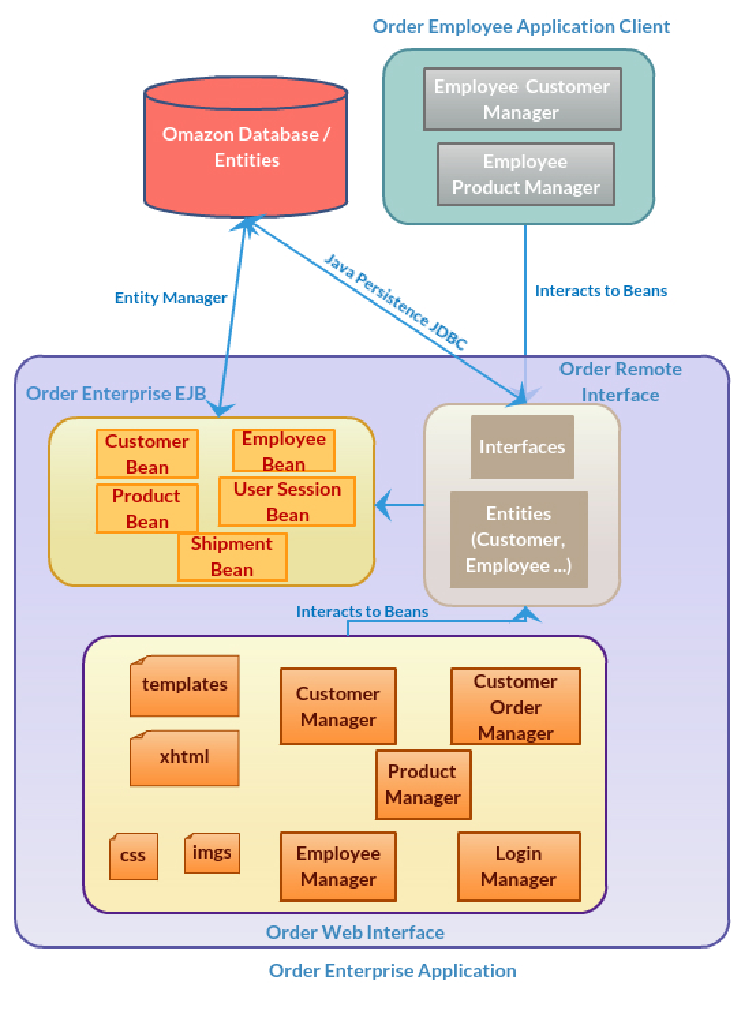
\includegraphics[width=85mm]{architecture}
   \caption{Omazon Architecture}
\end{figure}

The Employee application client and the user/employee web interface accesses the session beans, through the remote interface in the class library. The class library is accessed by the enterprise application (web interface) as well as the application client. The interaction between the various components is illustrated in the architecture diagram in Figure 1. 

  \subsection{Encountered problems/Implementation Alternatives}
\paragraph{Interaction between the models}
\begin{enumerate} \itemsep1pt \parskip0pt \parsep0pt
\item We encountered that our previous architecture could not fulfill the requirement of an native client.
To tackle this, we introduced the remote library for our business logic (beans), so that the interaction between the client and business logic could take place.
\item  Now, interaction with the database via Java Persistence required importing existing entities from the database to the remote interface.
Further communication of JavaEE persistence $Entity\_Manager$ required using JavaEE 7.
So, we proceed using JavaEE 7 libraries for our project.
\item In addition to this, the interaction between the entities, primary key <-> foreign key, in the logic was a problem. Earlier we did not really took care of the relationships between models what we now had to add. The first point where we needed this was displaying the current customers orders on the web interface without writing a manual filter over all existing orders but using a $WHERE$ clause and a parameterized query. 
\end{enumerate}

\paragraph{Code Cleanup and Refactoring}
As already mentioned at several points, we started of with the basic example and often used the existing files as a reference. Now, as the project has grown, we realized that we have to refactor a lot to keep the overall code base and therefor the effort of debugging and also implementing new features low.

\paragraph{JSF/JSP different then "normal" Web Development}
Compared to Web Development known to us from the PHP and Python world, JSP behaves much more like a native client framework and contradicts the way we used to think about web application and known practices in their development.

 \subsection{Implemented features}
As illustrated in the architectural overview, the design contains an enterprise application with the necessary business logic of adding/editing customer/product data and the order process. The $Employee$ application client can also add/edit the customer and product data by accessing the same business logic. As per the business logic, the user or the $Customer$ can login and order a product/multiple products. The corresponding $Order$ details of the customer is stored in the database, and the $shipment\_ID$ is automatically generated for the order. The $Status$ is then marked by the $Employee$. $Customer$ is then able to check the status via the web interface.

\subsubsection{Java Native interface for Employee}
Employee application client interacts to the session beans via Java class library. This displays the current list of products and customers to the employee. He can add or edit new data into the current list which is then synchronized with the Omazon Inc. database. The client functions can be seen in Figure 2.

\begin{figure}[h!]
  \centering
   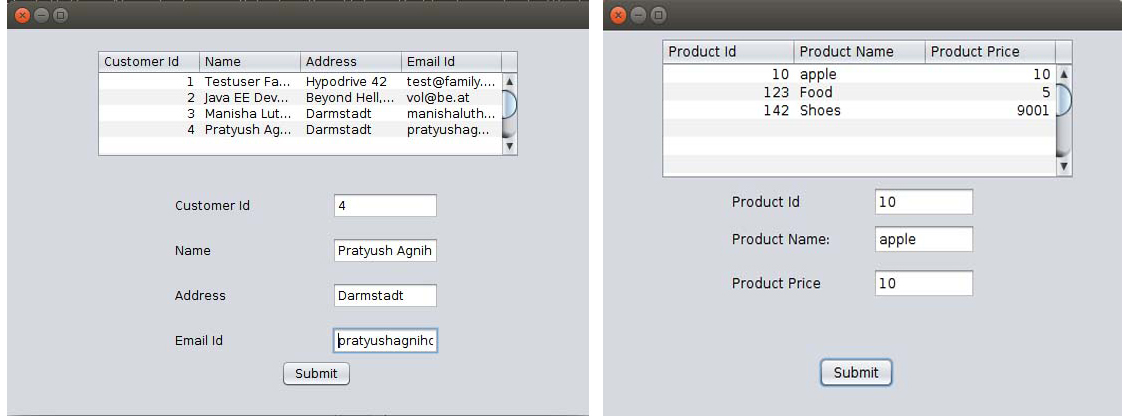
\includegraphics[width=150mm]{native}
   \caption{Java native client for Employee}
\end{figure}

\subsubsection{Order Process Support}
The functions of customer and employee user interface can be seen in Figure 3 and 4.
\begin{figure}[h!]
  \centering
   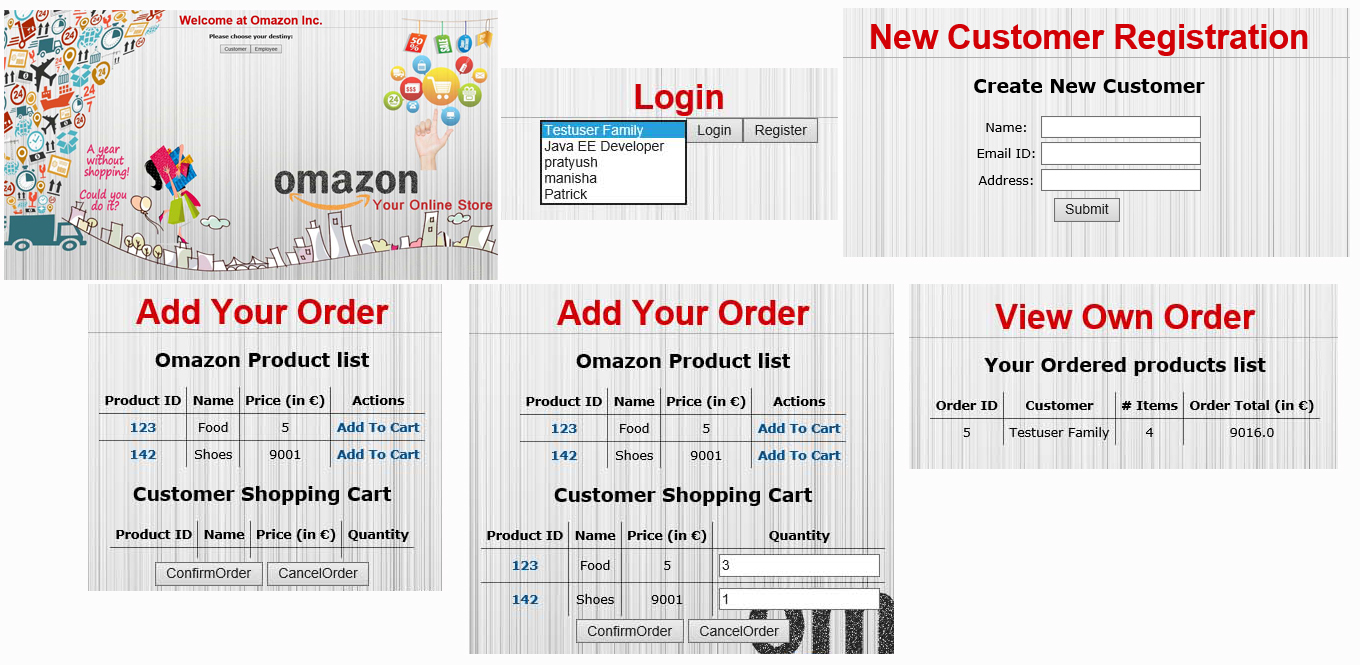
\includegraphics[width=150mm]{customer}
   \caption{Customer Interface}
\end{figure}

\begin{figure}[h!]
  \centering
   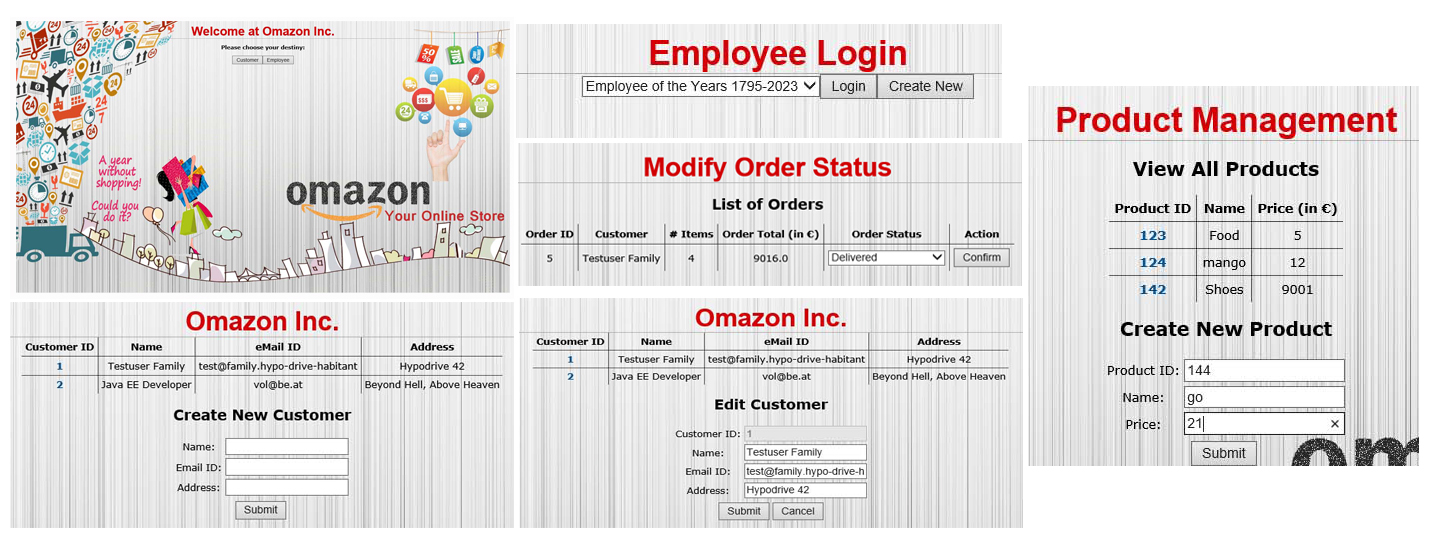
\includegraphics[width=150mm]{employee}
   \caption{Employee Interface}
\end{figure}

\begin{enumerate}\itemsep1pt \parskip0pt \parsep0pt
\item \textbf{Order Process:}
Customer can add one or more products from the product list to his cart, which is only saved in a SessionScoped Manager.
Once confirmed, the Order and an according Shipment is created in the database.
The user has the possibility to see a summary of his order including the current shipment status.
\item \textbf{Shipment Status update:}
Customer can check the status of his placed order via the web interface. 
The Employee can update the status of all orders.
\item \textbf{User Interface:}
The $CustomerManager$, $CustomerOrderManager$ and so on, the $ManagedBeans$, handles the communication and display the successful order table to the customer and the employee.
\end{enumerate}
\end{document}
